\section{Обзор взаимодействия}\label{COMMON.Overview}

Взаимодействие сторон инфраструктуры представлено на 
рисунке~\ref{Fig.COMMON.Bias}.

Пользователь регистрируется в инфраструктуре с помощью РЦ. При регистрации
проводится сбор идентификационных данных пользователя. Эти данные РЦ пересылает 
СИ. СИ передает их в управление СР вместе с другими ресурсами пользователя.

Обычно при регистрации подтверждается личность пользователя, в том числе 
проверяется корректность собранных идентификационных данных. Подтверждение 
личности основано на проверке удостоверений пользователя.

Подтверждение личности может не проводиться. Например, допускается, что пользователь
указывает при регистрации самозаявленные (никем не подтвержденные) имя и
фамилию. Регистрация без подтверждения личности проводится напрямую между
пользователем и СИ.

\begin{figure}[hbt]
\begin{center}
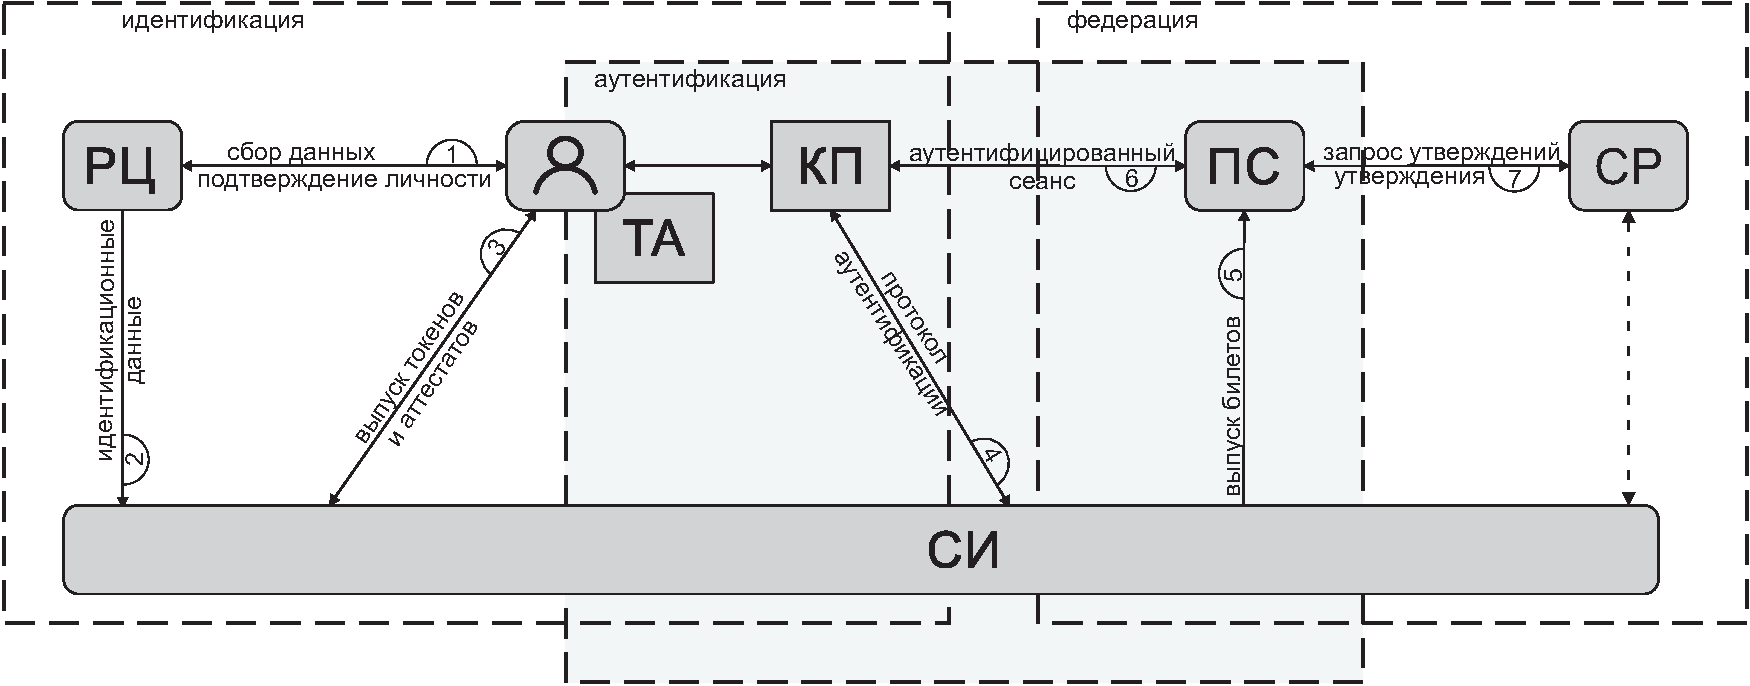
\includegraphics[width=17cm]{../figs/bias}
\end{center}
\caption{Взаимодействие сторон инфраструктуры}
\label{Fig.COMMON.Bias}
\end{figure}

% СИ завершает идентификацию пользователя, назначая ему уникальный 
% идентификатор. Он может быть выбран пользователем (логин, псевдоним) или 
%согласован с пользователем.

В ходе регистрации пользователь и СИ согласуют перечень ТА, которые будут 
использоваться при аутентификации. СИ хранит информацию о связи между 
пользователями и его токенами в аттестатах.

СИ по запросу ПС, инициированному обращением пользователя, проводит
аутентификацию пользователя. В ходе аутентификации пользователь доказывает
владение одним или несколькими токенами, указанными в аттестате.
%
В случае успеха СИ выдает ПС билеты: аутентификации (БА) и доступа (БД). 
%
БА подтверждает подлинность пользователя и может быть использован
для открытия ему доступа к ресурсам ПС.
%
БД авторизует ПС перед СР на доступ к ресурсам пользователя.

Кроме двух основных билетов, могут использоваться дополнительные.
Например, билет обновления позволяет организовать перевыпуск других билетов
без повторной аутентификации. Билет сеанса позволяет организовать 
аутентифицированный сеанс между пользователем и ПС.

Для доступа к услугам аутентификации и авторизации ПС предварительно 
регистрируется в СИ как член федерации.


